\documentclass{article}

% set font encoding for PDFLaTeX or XeLaTeX
\usepackage{ifxetex}
\ifxetex
  \usepackage{fontspec}
\else
  \usepackage[T1]{fontenc}
  \usepackage[utf8]{inputenc}
  \usepackage{lmodern}
\fi
\usepackage{graphicx}

% used in maketitle
\title{Actividad 5}
\author{Jesús Adrián Zatarain Alvarado}
\date{6 de marzo del 2018}

% Enable SageTeX to run SageMath code right inside this LaTeX file.
% documentation: http://mirrors.ctan.org/macros/latex/contrib/sagetex/sagetexpackage.pdf
% \usepackage{sagetex}

\begin{document}
\maketitle

\section{Introducción}

En esta práctica se tiene como objetivo el conocimiento del uso de ciertos comandos de emacs. Se continúa desde donde se dejó la actividad anterior, con los datos recolectados. Se hará uso intensivo de comandos de recortes para filtrar ciertas palabras. Al final se analizará el archivo en Pandas y se realiarán algunas gráficas relacionadas a los datos filtrados. En total se tendrán dos archivos; uno con los datos de cierta hora del día y otros con otra.

\section{Descripción de los conceptos físicos de CAPE y PW, que se obtienen de los datos de sondeos de la parte alta de la atmósfera.}

Las siglas CAPE (Convective Available Potential Energy) hacen referencia a la energia potencial disponible para la convección en un momento dado. Se trata de uno de los parámetros convectivos más interesantes de todos aquellos que se derivan de los modelos meteorológicos y por este motivo lo intentaremos explicar a lo largo de las siguientes líneas.

Es importante empezar remarcando que se trata de un parámetro que nos indica cuanta energía está disponible para la convección en caso de que esta se inicie. Por lo tanto, la consulta de este parámetro se tiene que complementar siempre con la lectura de otros campos del modelo que nos permitan determinar la probabilidad de que la convección se inicie. De hecho, es muy habitual que en los distintos portales meteorológicos se pueda ver ya combinado con otro tipo de información. 

El agua precipitable es la cantidad de agua, expresada como altura o masa, que se obtendría si todo el vapor de agua contenido en una columna específica de la atmósfera, de sección transversal horizontal unitaria, se condensase y precipitase.

\section{Descripción del proceso de limpieza y preparación de los datos para posteriormente analizar con Pandas.}

Del archivo obtenido de la actividad anterior, se prosiguió a seleccionar sólo las columnas que coincidieran con las palabras clave "CAPE" y "Precipital Water (PW)", donde creó un archivo con esas variables más la fecha en que fueron recolectados los datos, y también muchos datos que venían por defecto en él.

Tenían los siguientes datos antes de que se filtrará CAPE y PW:

\begin{figure}[h!]
  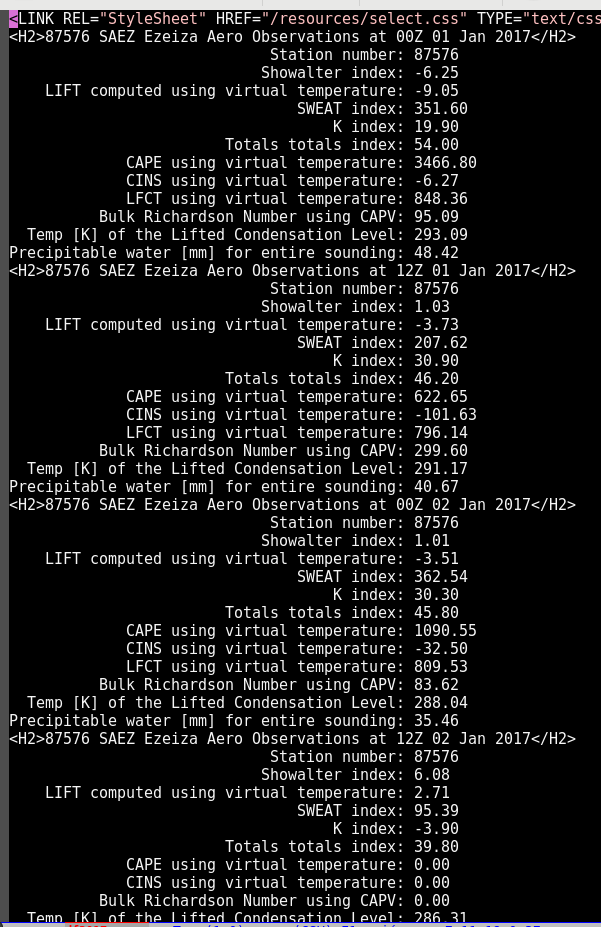
\includegraphics[width=11cm, height=11cm]{original.png}
  \caption{}
  \label{}
\end{figure}

\newpage

Lo siguiente consiste en borrar los datos no necesarios para la siguiente parte de la actividad. Sólo se necesitan el CAPE, PW, y la fecha, al igual que su correspondiente hora del día a la que fueron tomados los datos.


Para seleccionar sólo CAPE y PW, se usó el comando:

\begin{verbatim}

~$ egrep -v 'PRES|hPa' df2017_2.csv | egrep '76225|CAPE|Precip' > df2017_PWs.csv

\end{verbatim}

Que sólo filtrará las palabras claves entre comillas y crea un archivo a partir de otro archivo, el nuevo archivo tendrá sólo los carácteres seleccionados.

Posteriormente, se inciará el proceso de eliminación de texto innecesario en el archivo nuevo, por medio del editor Emacs. Se usarán los comandos intrínsecos en él, que sirven para guardar carácteres en la memoria volatil, la reemplazación de letras por otras y la utilización de un comando que sirve para aplicar los mismo para todos los demás carácteres de la misma condición. Los comandos utilizados están descritos a continuación:

\begin{itemize}

\item Control-W: Sirve para guardar el texto seleccionado en la memoria para su posterior utilización

\item Control-Y: Se usa para desplegar el texto guardado en la memoria en una parte en específico.

\item Esc-shift-5: Sirve para entrar en un modo, donde lo que se encuentra después de éste, puede ser reemplazado por los carácteres que el usuario introduzca por otros a su placer.

\item shift-1: La acción a realizar se hace íntegramente en todos los demá de su condición.

\end{itemize}

Al final el archivo lucirá así:

\begin{center}
  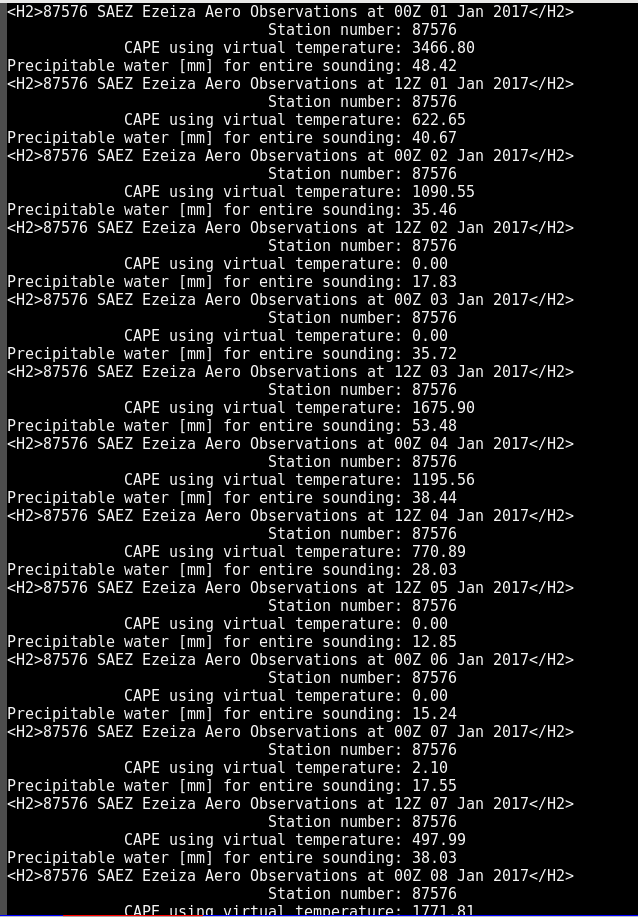
\includegraphics[width=11cm, height=11cm]{CAPEPW.png}

\end{center}

Después, se separará el archivo en dos, cada uno con una hora diferente del día. Para ello se utiliza el comando grep como sigue a continuación:

\begin{verbatim}

~$ egrep -v '00Z' df2017_2.csv > df2017_PW_12Z.csv


\end{verbatim}

Que recortará todas las lineas que coincidan con "00Z" en el archivo. Lo que quede en el archivo se colocará en un nuevo archivo que se usará más adelante.
Para los correspondientes a "12Z", se prosigue a realizar casi lo mismo; sólo que se cambia las palabras clave y el nombre del archivo para su diferenciación y no se reemplaze por el anterior creado.

\begin{verbatim}

~$ egrep -v '12Z' df2017_2.csv > df2017_PW_00Z.csv


\end{verbatim}

Ya con los dos archivos creados, filtrados y listos para usarse; se prosigue a crear una sesión en Jupyter notebook donde se analizará el archivo por medio de bibliotecas del lenguaje Python.

\begin{center}

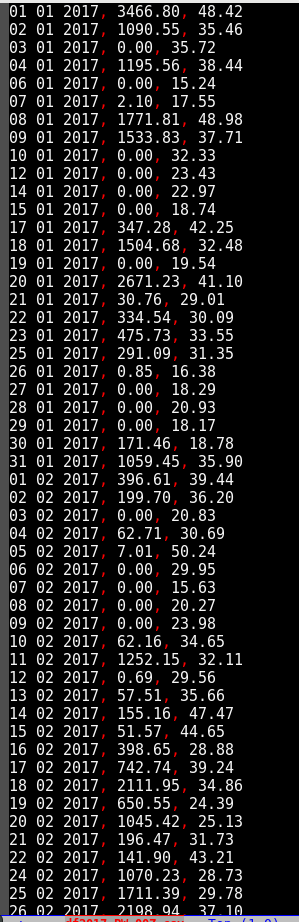
\includegraphics[width=4cm, height=6cm]{final.png}

\end{center}


\section{Análisis de datos utilizando Pandas}

Para el análisis y creación de gráficas, se utilizó la biblioteca Pandas, que permite analizar archivos de texto. Se usó el código proporcionado por el docente para poder realizar lo faltante de la actividad.

\begin{center}
  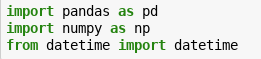
\includegraphics[width=4cm, height=1cm]{inicio.png}
\end{center}



Que contiene las bibliiotecas que se usarán en la actividad. Está la biblioteca de pandas, que es para el análisis del archivo, numpy para el maneo de datos, y por último, datetime, que permite manejar las fechas contenidas en el archivo.

\begin{center}
  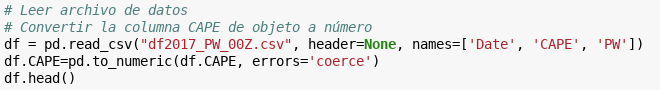
\includegraphics[width=4cm, height=2cm]{leer.png}
\end{center}

Esta parte lee el archivo en cuestión. Se tiene que introducir el nombre del archivo con su correspondiente extensión. Despliega cinco lineas del archivo para verificar si lo ha leído correctamente.

\begin{center}
  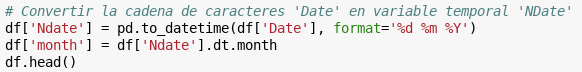
\includegraphics[width=4cm, height=1cm]{convertir.png}
\end{center}

Que toma los datos correspondientes a las fechas y los hace utilizables en el posterior análisis y gráficas a realizar.

Ahora se pasa a la parte de graficar los datos, para poder observar su distribución. En la primera se tiene el siguiente código:

\begin{center}
  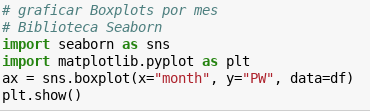
\includegraphics[width=4cm, height=1cm]{PWbot.png}
\end{center}

EL cual va a desplegar una gráfica que contiene los datos registrados de agua precipitada por mes.
Los siguiente en la actividad es la realización de una gráfica de PW contra CAPE, que tiene todos los datos en forma de puntos en la gráfica, al igual que una recta con ajuste lineal.

\begin{center}
  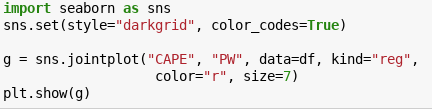
\includegraphics[width=4cm, height=1cm]{dispersos.png}
\end{center}

Al final se hizo una gráfica de con el comando: sns.lmplot, para hacer la gráfica correspondiente.


\section{Resultados del análisis}

Se leyeron los dos archivos para poder realizar las gráficas correspondientes.

La primera fue por medio de boxplot. En primera, se tiene a los datos correspondientes a 00Z ,seguidos de los 12Z.
Las gráficas a continuación son para el CAPE. Las dos son diferentes, y se presetan en forma de caja.

\begin{center}
  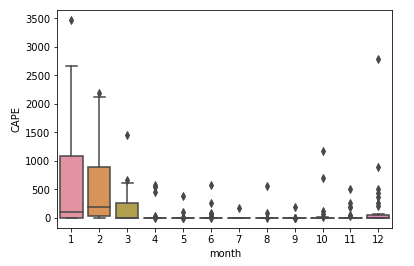
\includegraphics[width=6cm, height=6cm]{CAPEbotGrafica.png}
\end{center}

\begin{center}
  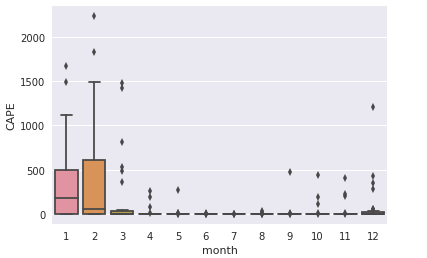
\includegraphics[width=6cm, height=6cm]{CAPEboxGraficaZ.png}
\end{center}

En la siguiente, se tienen los datos correspondientes a el agua precipitada por mes para cada uno. 

\begin{center}
  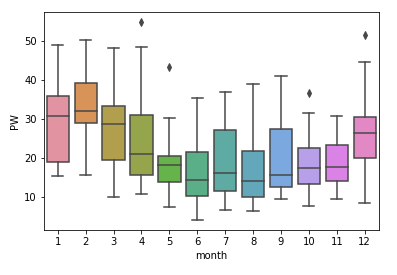
\includegraphics[width=6cm, height=6cm]{PWbotGrafica.png}
\end{center}

\begin{center}
  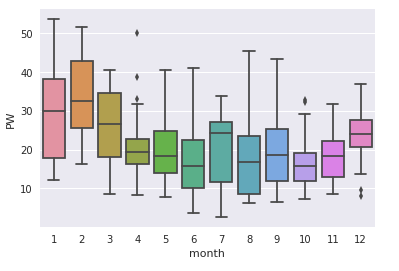
\includegraphics[width=6cm, height=6cm]{PWboxGraficaZ.png}
\end{center}

Las dos gráficas a continuación se asemejan mucho. Son gráficas de PW contra CAPE que muestran los datos en forma de puntos y hace un ajuste lineal de ellos. En la parte superior se tiene el CAPE respecto al timepo, al lado derecho el PW respecto al timepo, su distribución
\begin{center}
  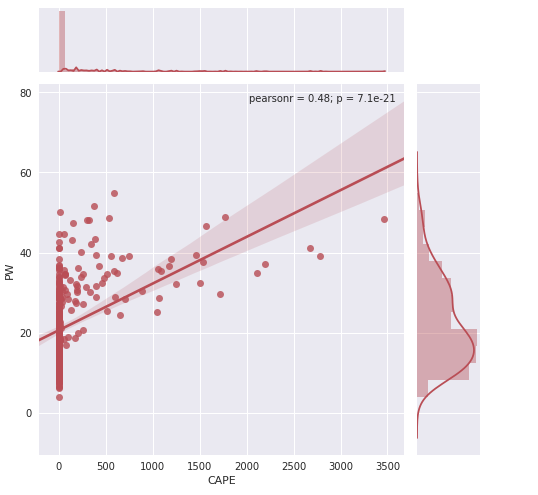
\includegraphics[width=6cm, height=6cm]{dispersosGrafica.png}
\end{center}

\begin{center}
  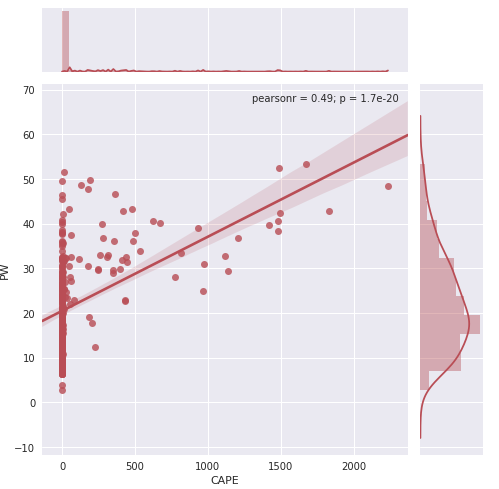
\includegraphics[width=6cm, height=6cm]{dispersosGraficaZ.png}
\end{center}

Por último se tienen estas dos gráficas. Muestran la dispersión de los datos por medio de los triángulos tenuez.

\begin{center}
  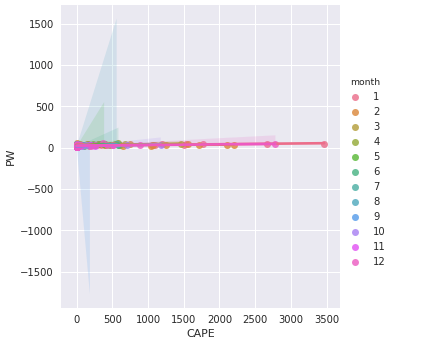
\includegraphics[width=6cm, height=6cm]{JuntosGraf.png}
\end{center}

\begin{center}
  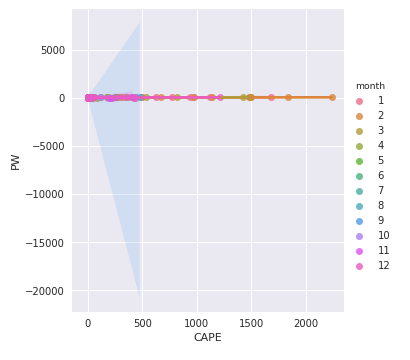
\includegraphics[width=6cm, height=6cm]{juntosGraficaZ.png}
\end{center}


\section{Conclusiones}

Fue una práctica donde se aprendió mucho sobre los comandos de Emacs, que puede servir para recortar caráteres con patrones similares, y hacer los recortes necewsarios para poder utilzar los datos correspondientes con más facilidad. También se vio un poco sobre graficación de datos, que desplega una nueva forma no conocida hasta entonces por el estudiante.

\section{Bibliografía utilizada}

http://www.meteoillesbalears.com/?p=623

\section{Apéndice}

¿Cómo se te hizo esta actividad? ¿Compleja, Difícil, Sencilla?

Fue sencilla, pero tardada; más por los nuevos comandos que se aprendieron.
\\
\\
¿Qué te llamó más la atención?

La fácil utilización de Emacs para la manipulación de archivos. Al igual que las distintas gráficas que se hicieron.
\\
\\
¿Qué parte fue la que menos te interesó hacer?

Todo estuvo bien
\\
\\
¿Cómo mejorarías esta actividad? ¿Qué le faltó? ¿Qué sobró?

Fue buena actividad, no le faltó nada
\\
\\
¿Hasta este punto, que te parece el uso de Jupyter para programar en Python? 
Es una buena herramienta que siempre puedes tener disponible.

\end{document}
